\documentclass{pracamgr}  
\usepackage{lmodern} 
\usepackage[polish]{babel} 
\selectlanguage{polish} 
\usepackage{fontspec}
\usepackage{minted}
\usepackage{listings}
% package for hyperinks
\usepackage{hyperref}
\hypersetup{
    colorlinks,
    citecolor=black,
    filecolor=black,
    linkcolor=black,
    urlcolor=black
}
\usepackage{graphicx}  
\usepackage{makeidx}\makeindex
 
\definecolor{grey}{gray}{0.9}
\definecolor{bg}{HTML}{FAFAFA}
\definecolor{darkgray}{HTML}{D5D5D5}

\makeatletter
\renewenvironment{minted@colorbg}[1]{
\setlength{\fboxsep}{\z@}
\def\minted@bgcol{#1}
\noindent
\begin{lrbox}{\minted@bgbox}
\begin{minipage}{\linewidth}}
{\end{minipage}
\end{lrbox}%
\colorbox{\minted@bgcol}{\usebox{\minted@bgbox}}}
\makeatother

%Jesli uzywasz kodowania polskich znakow ISO-8859-2 nastepna linia powinna byc odkomentowana
%Jesli uzywasz kodowania polskich znakow CP-1250 to ta linia powinna byc 
%odkomentowana
%\usepackage[cp1250]{inputenc}

% Dane magistranta:

\author{Konrad Lisiecki}
\nralbumu{48211}
\title{Wycena Opcji przy użyciu Modeli Zmienności Stochastycznej} 
\kierunek{Finanse i rachunkowość}
\instytut{Ekonometrii}
\opiekun{dra hab. Łukasza Delonga} 
\date{Warszawa 2015}   

% Tu jest dobre miejsce na Twoje własne makra i~środowiska:
\newtheorem{defi}{Definicja}[section]

% koniec definicji 

%\makeindex[intoc] 
 


%===========================================================================
%             Bibliogrphy
%=========================================================================== 
\usepackage[style=numeric,sorting=ydnt,defernumbers=true, backend=bibtex]{biblatex}
\addbibresource{biblio.bib}
 

%===========================================================================
%                           Begin of document 
%===========================================================================


\begin{document}
\maketitle
\nocite{book-full} 

%===========================================================================
%                               Introduction
%===========================================================================
\chapter*{Streszczenie} 

\begin{quote}
We developed what is known a stochastic volatility model. This is a model where the volatility as well as the underlying asset price moves around in an unpredictable way.
\raggedleft\slshape John Hull \index{Hull John}
\end{quote}



%===========================================================================
%                               Table of contents
%===========================================================================
\tableofcontents
 

\addcontentsline{toc}{chapter}{Introduction} \markboth{INTRODUCTION}{}


%===========================================================================
%                               Wprowadzenie
%===========================================================================
\chapter{Wprowadzenie}\label{r:pojecia}
\begin{quote}

Never think that lack of variability is stability. Don't confuse lack of volatility with stability, ever.
 
\raggedleft\slshape Nassim Nicholas Taleb \index{Taleb Nassim Nicholas}
\end{quote}
 


adsafdsdfs
 
\section{Definicje}
dsfdsf

\section{Systemy handlu algorytmicznego}


\section{Modele zmienności stochastycznej}
dsfdsf

\section{Proces formowania strategii inwestycyjnej}
Cały proces formowania strategii inwestycyjnej można ująć w 4 krokach:

\begin{enumerate}
\item 
\item modelowanie
\item walidacja modelu (ang. Backtesting)
\item analiza wyników 
\end{enumerate}

\section{Backtest}
Backtestem nazywamy symulację stworzonej strategii na danych. Dane te mogą
być danymi historycznymi lub sztucznie wygenerowanymi.

\section{Kointegracja}
dsfdsf

\begin{defi}\label{aa}
fsdf
\end{defi}

\begin{defi}\label{aaa}
sdfsdf
\end{defi}




%===========================================================================
%
%                               Model Hestona
%
%===========================================================================
\chapter{Inwestycje na rynku opcji}
\begin{quote}
  Suppose we use the standard deviation ... of possible future returns on
  a stock ... as a measure of its volatility. Is it reasonable to take
  that volatility as a constant over time? I think not.

\raggedleft\slshape Fisher Black \index{Fisher, Black}
\end{quote}


Obecnie jednym z najpopularniejszych narzędzi do wyceny opcji jest model Blacka-Scholsa. Ceniony jest on ze względu na prostotę oraz wygodę użycia, kosztem jednak wielu upraszczających założeń. 


\section{Motywacja} 
Jak zostało powiedziane we wstępie do niniejszego rozdziału, podstawowym modelem do wyceny opcji jest model Blacka-Scholesa.
Umożliwia on wyprowadznie wzroru na cenę opcji europejskiej w postaci analitycznej. Jednakże, podczas gdy jego prostota jest jedną z jego największych zalet, to posiada on wiele założeń, które nie przystają do rzeczywistości rynkowej. Pierwsza grupa to założenia dotyczące aktywów:
\begin{enumerate}
\item cana aktywów bazowych ma rozkład lognormalny
\item zmienność aktywów bazowych ijest stała i znana z góry
\item akcje nie wypłacają dywidend
\item wyceniane opcje są opcjami Europejskimi, tzn. przy pomocy modelu Blacka-Scholesa nie można wycenić np. opcji Amerykańskich
\end{enumerate}
Z kolei druga grupa założeń odnosi się do rynku na którym dane aktywa występują.
\begin{enumerate}
\item na rynku nie ma możliwości osiągnięcia ponadnormatywnego zysku bez ryzyka (brak możliwości arbitrażu)
\item nie ma kosztów transakcyjych
\item stopa procentowa na rynku $r_t$ jest stała i znana z góry 
\end{enumerate}

Wszystkie te założenia sprawiają, że model Blacka-Scholesa, mimo, że pozwala na wyznaczenie ceny opcji w postaci analitycznej, może nieprecyzyjnie wycenić wartość takiej opcji.
Jednym z takich założeń jest to o stałej zmienności instrumentu bazowego. Jednym z pomysłów na obejście tego problemu jest uzmiennienie tej stałej, czyli pozwolanie, aby dla dowolnego czasu, parametr ten przyjmował różną wartość. Można to zrobić np. poprzez nadanie zmienności cech losowych. W takim przypadku nie tylko proces ceny akcji byłby procesem stochastycznym, ale także aby sama zmienność byłaby definiowana przy użyciu procesu stochastycznego. Takie też podejście zostało wykorzystane przy budowie modelu Hestona. \cite{greenwade93}


\section{Model Blacka-Scholesa}

Jak zostalo wspomniene we wstepie podstawowym modelem matematycznym na wycenę opcji jest model Blacka-Scholesa. Najczęściej definiuje się go w następującej postaci:
\begin{equation}
dS_t  = \mu S_t dt + \sigma S_t dW^S_t
\end{equation}

We wzorze tym $S_t$ przedstawia cenę instrumentu bazowego w momencie $t$, stała $\mu$ oznacza dryf, stała $\sigma$ oznacza zmienność, natomiast $dW^S_t$ jest standardowym procesem Wienera.


Ze względu na swoją prostotę, model ten jest podstawową metodą do wyceny opcji, jednak wspomniana prostota niesie za sobą szereg ograniczeń. Jednym z takich ograniczeń jest założenie o stałej wartości zmienności w czasie. Jak bardzo to założenie potrafi być niezgodne z rzeczywistością pokazał chociażby ostatni kryzys finansowy, podczas którego zmiennośc instrumentów finansowych była o wiele większa niż w poprzednich latach. Dlatego też naturalnym uogónieniem modelu Blacka-Scholesa wydaje się być wprowadzenie zmienności, która w rzeczywistym świecie nie jest stała. Taką zmianę wprowadza model Hestona. 


\section{Model Hestona}
Jak wspomniano w poprzednim rozdziale, model Hestona eleminuje podstawową wadę modelu Blacka-Scholesa jakim jest założenie o stałej zmienności w czasie.
W tym celu zmienność również uzależniono od procesu losowego, tworząc kolejny proces stochastyczny. W przypadku modelu Hestona jest to model Coxa-Ingersolla-Rossa (model CIR):
\begin{equation}
dr_t  = \kappa (\theta  - r_t)dt + \epsilon \sqrt{r_t} dW_t^v 
\end{equation}

Model CIR jest często wykorzystywany przy modelowaniu zmienności stopy procentowej (stąd też oznaczenie $r_t$) ze względu na \textbf{\textit{własość powrotu do średniej długoterminowej}}. 
(\textit{ang. mean-reversion}). Gdy zamiast $r_t$ podstawimy $v_t$ otrzymamy proces przedstawiający zmienność zmienności w czasie. Tak jak w przypadku stopy procentuwej, tak w przypadku akcji występuje własność powrotu do średniej, gdy cena akcji nie spadnie poniżej 0 \cite{TestingMeanReversion}.
Co więcej, gdy proces spełnia warunek Fellera:
\begin{equation}
2 \kappa \theta > \epsilon^2
\end{equation}
proces jest ściśle dodatni \cite{TheLittleHestonTrap}.


Co więcej zmienność jest zawsze jest wartością większą od zera, co wynika wprost z jej definicji. Stąd też w drugiej części wzoru mamy funkcję pierwiastkową z $v_t$: 

\begin{equation} 
dv_t  = \kappa (\theta - v_t)dt + \epsilon \sqrt{v_t} dW_t^v 
\end{equation}

Mając równanie opisujące proces zmienności można już przedstawić model Hestona, który ma postać:

\begin{equation}
dS_t  = \mu S_t dt + \sqrt{v_t} S_t dW^S_t
\end{equation}

\begin{equation}
dv_t  = \kappa (\theta - v_t)dt + \epsilon \sqrt{v_t} dW_t^v 
\end{equation}

\begin{equation}
Cov[dW^S_t, dW^v_t] = \rho dt 
\end{equation}
gdzie:
\begin{enumerate}
\item $\mu$ oznacza dryft (\textit{ang. drift}). ceny aktywa bazowego 
\item $\theta$ oznacza długoterminową wartością oczekiwaną $v_t$
\item $\kappa$ jest współczynnikiem szybkości powrotu do średnej (\textit{ang. rate of mean-reversion})
\item $\epsilon$ oznacza zmienność zmienności, czyli warinację $v_t$
\end{enumerate}

W dodatku, w przedstawiony modelu występuje równanie $Cov[dW^S_t, dW^v_t] = \rho dt $. Mówi ono o tym, że 
dwa procesy błędzenia losowego są w rzeczywistości ze sobą skorelowane przy pomocy stałego współczynnika 
korelacji $\rho$.

Niestety, w odróżnieniu od modela Blacka-Scholsa, dla modelu Hestone nie istnieje pełne rozwiązanie analitycznie (istnieje tylko częściowe rozwiązanie analityczne). Wobec tego, aby należy się posłużyć numerycznymi metodami wyznacznia rozwiązania.

% Poniższa lista przedstawia podstawowe 
% \begin{enumerate}
% \item rozkłąd logarytów stóp zwortu nie jest normalny
% \item zmienność jest zmienna w czasie
% \item autokorelacja kolejnych stóp zwrotu
% \item trajektorie mają skoki
% \end{enumerate}

% W kolejnych rozdziała 








% %===========================================================================
% %                               Model Hestona
% %===========================================================================
% \section{Model Hestona}

% Na początek załóżmy, że cena aktywa bazowego w momemcie $t$ spełnia następujący proces dyfuzji:
% \begin{equation}
% dS(t)= \mu S dt + \sqrt{v(t)} S d z_1 (t),
% \end{equation}
% gdzie $z_1(t)$  jest standardowym procesem Wienera. 

% Jeżeli natomiast zmienność jest procesem Ornsteina-Uhlenbecka:

% \begin{equation}
% d \sqrt{v(t)} = - \beta \sqrt{v(t)} dt + \delta d z_2 (t)
% \end{equation}

% wtedy na podstawie lematu Ito można wykazać, że wariancja $v(t)$ ma nastepującą postać:
% \begin{equation}
% dv(t)= \kappa  [\theta -v(t)]dt+2\delta \sqrt{v(t)} d z_2 (t)
% \end{equation}
% gdzie proces $z_2(t)$ ma korelację z procesem $z_1(t)$ równą $\rho$.

% Gdy przyjmiemy stałą stopę procentową, cena w momencie $t$ obligacji, która wygasa w chwili $t+\tau$ wynosi:
% \begin{equation}
% P(t, t+\tau) = e^{-r\tau}
% \end{equation}



% \begin{figure}
%   \centering
%   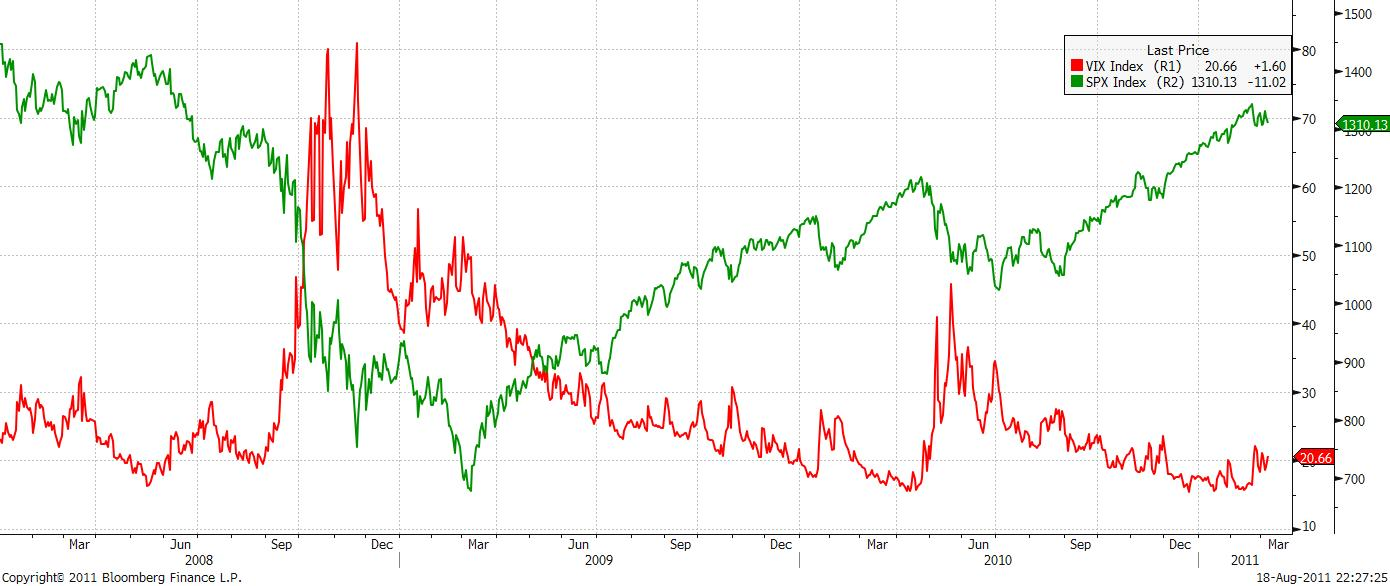
\includegraphics[width=150mm]{vix.jpg}
%   \caption{Zmieność w czasie indeksu S\&P}\label{fig:vix}
% \end{figure}


% gdzie parametr $\sigma$ jest stały. Założenie to jednak okazuję się być zbyt upraszczające dla szerokiej gamy szeregów czasowych. Spojrzmy np. na szereg czasowy  (\ref{fig:vix}) 



% \begin{equation}\label{h:ito}
% dv(t) = [\delta^2 - 2 \beta v(t)] dt + 2\beta \sqrt{v(t)} dz_2(t),
% \end{equation}

% The (\ref{h:ito}) equation can be rewritten to the following, square root process

% \begin{equation}\label{h:squareroot}
% dv(t) = \kappa [\theta - v(t)] dt + \sigma \sqrt{v(t)} d_2 (t),
% \end{equation}

\section{Metody Monte Carlo}

Poprzendni rozdział zakończono stwierdzeniem, że nie istnieje możliwość znalezienia dokładnego rozwiazania analitycznego
dla modelu Hestona. Z tego względu stosuje się następujące metody numeryczne:
\begin{enumerate}
\item 
\end{enumerate}

\section{Dyskretyzacja Eulera}

Po

 Jak wynika ze wzorów  
\begin{equation}\label{h:euler}
v_{i+1}  = v_i + \kappa (\theta - v_i) \Delta t + \epsilon +  \sqrt{v_i} \Delta W^{v}_{i+1}
\end{equation}
  
\section{Generowanie skorelowanych szeregów czasowych}
W tej sekcji zajmiemy się generowanie skorelowanych szeregów czasowych o zadanym stopniu korelacji $\rho$.
Jednym z ważniejszych zagadnienień związanych z użyciem modelu Hestona jest odpowiednie generowanie skorelowanych szeregów czasowych. Algorytm , przedstawiony w zaloaczniku do pracy opisuje, jak majac dwa kontenery z wartościami z rozkładu jednostajnego możemy wygenerować nowy wektor o zadanej korelacji $\rho$ w stosunku do pierwszego kontenera z danymi. 

Poniższy wykres przedstawia wygenerowane przekladowe szeregi czasowe z zadanym poziomem korelacji na poziomie $\rho = 0.2$:

\begin{figure}
  \centering
  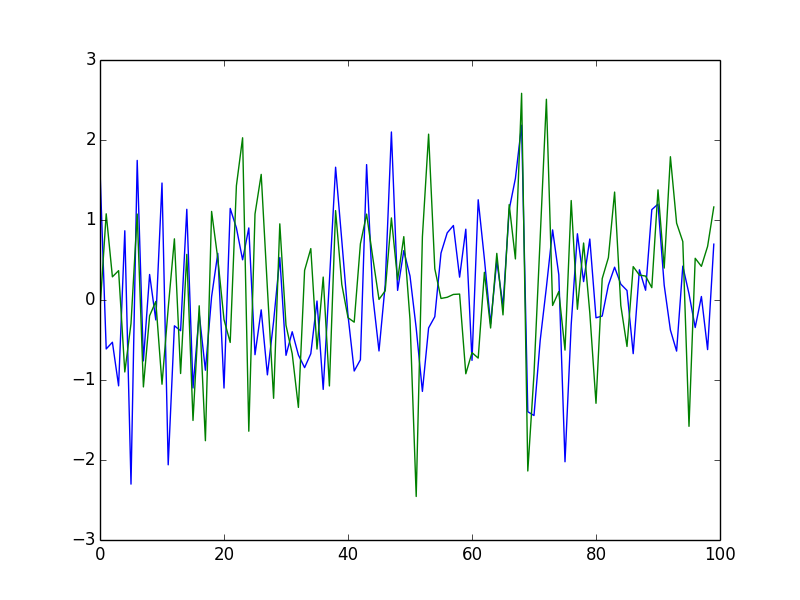
\includegraphics[width=150mm]{corr.png}
  \caption{Zmieność w czasie indeksu S\&P}\label{fig:vix}
\end{figure}

Majac w ten sposób wyznaczone szeregi czasowe o zadanym poziomie korelacji teraz przychodzi czas na generowanie szeregu czasowego opisujacym zmienność oraz samą cenę instrumentu finansowego. 
Przypomnijmy, że zgdonie z modelem Hestona wzory te prezentują się następujuąco:

Mając funkcje generujacą skorelowane szergi czasowe mozna zdefiniowac funkcje, ktorej wynikiem bedzie cena instrumentu bazowego w danej chwili. Jej definicja będzie zgodna z następujacym zbiorem formul: \cite{OptimalInvestment2010}

\begin{equation}
dS_t =  \mu S_t  dt + \sqrt{V_t}S_t dW_t^1
\end{equation}

\begin{equation}
dV_t =  \kappa (\theta - V_t)  dt + \sqrt{V_t} dW_t^2
\end{equation}

\begin{equation}
dW_t^1 dW_t^2  = \rho dt
\end{equation}


%===========================================================================
%                       Kalibracja modelu Hestona
%===========================================================================
\chapter{Kalibracja modelu}


Mając wyznaczony dla którego chcielibyśmy wyznaczyć cenę opcji, wciąż potrzebujemy parametrów dla tego modelu. 
Problem wyznaczenia parametrów modelu nazywamy \textbf{problemem kalibracji} modelu.  

Cena opcji, która jest wynikiem symulacji w modelu Hestona jest 

Jednym ze sposobem na kalibrację modeli jest technika symulowanego wyżarzania (ang. simulated annealing). Należy od do 
grona stochastycznych metaheurystyk, które pomagają w rozwiązaniu problemów optymalizacyjnych (a takim właśnie problemem jest
kalibracja modelu)



\section{Symulowane Wyżarzanie}

Tematem tego podrozdziału jest algorytm symulowanego wyżarzania  (\textit{ang. simulated annealing}). 

Podstawowym problem podczas rozwiązywania problemów optymalizacyjnych jest istnienie wielu ekstremów lokalnych.
W tym przypadku większość algorytmów, które są monotoniczne, nigdy nie osiągnie ekstremum globalnego. Jedną z takich technik jest \textit{hill climbing}, która osiąga dobre rezultaty tylko dla funkcji wypukłej powierzchni.
Aby znaleść rozwiązanie tego problemu odchodzi się od zasady monotoniczność, tzn. algorytm nie zawsze wybiera rozwiązanie bardziej optymalne od poprzedniego. 
Wśród możliwych podejść należy wymienić np.:
\begin{enumerate}
  \item pełny przegląd badanego obszru
  \item podejście determinstyczne w algorytmie \textit{tabu search}
  \item podejście randowmizacyjne (\textit{algorytm Metropolisa, symulowane wyżarzanie} \cite{OptimalizationBySimulatedAnnealing} )
\end{enumerate}


\begin{listing}[H]
\inputminted[mathescape, linenos, numbersep=5pt, bgcolor=bg, frame=lines, framesep=2mm]{python}
{listings/sa.py}
\caption{Przykład użycia funkcji anonimowejs}
\label{lst:lambdaSyntax}
\end{listing}
%===========================================================================
%                       Rozszerzenia modelu Hestona
%===========================================================================
\chapter{Rozszerzenia modelu Hestona}

Model Hestona, jak opisano w poprzednim rozdziale, odrzuca założenie o stałości zmienności w czasie. Jednak pozostałe parametry wciąż pozostają na nie zmienionym poziomie, 
co sprawia, że wprowadzono wiele jego rozszerzeń. 





% %===========================================================================
% %                       Model Hestona na przykładznie
% %===========================================================================
% \chapter{Optymalne decyzje inwestycyjne}\label{r:sp}
% Jak wiadomo zmienność nie jest bezpośrednio obserwowalna na rynkach finansowych.
% Aby wnioskować o zmienności, można:
% \begin{enumerate}
% \item wykorzystać technikę filtrowania (ang. filtering)
% \item ceny opcji z rynku lub indeksy zmienności rynkowej (ang. market volatility indices)
% \end{enumerate}

% Ustalająć $\mu =\frac{1}{2}$ 
% Gdzie parametr $\mu$ oznacza wrażliwość współczynnika dyfuzji względem poziomu zmienności.


% \begin{enumerate}
% \item Rozszerzony model Hestona z procesem CEV (ang. constant elasticity variance):

% Model CEV wyraża się przy pomocy następującego wzoru:
% \begin{equation}
% dS = \mu S dt  + \sigma_0 S^{\frac{}{}}
% \end{equation}

% Zmienność jest więc w tym przypadku funkcją ceny akcji (stochastycznej).


% \begin{equation}

% dV_t = k_V(\hat{V}-V_t)dt+ \hat{V}^{\frac{1}{2}-\mu} V_t^{\mu} (b_{SV} dB_t^S+ h_VdB_t^V)
% \end{equation}
% \item ceny opcji z rynku lub indeksy zmienności rynkowej (ang. market volatility indices)

% \item Rozszerzony model Stein-Steina (ang. extended Stein-Stein model):

% Równanie:

% \begin{equation}
% \frac{dS_t}{S_t} = (R_t + \lambda_t \sigma_t) dt + \sigma_t + d B_t^S
% \end{equation}

% \begin{equation}
% d\lambda_t  = \kappa_{\lambda} (\hat{\lambda} - \sigma_t) dt 
% + \beta_{\lambda S} dB_t^S + g_{\sigma}dB_t^{\sigma}
% \end{equation}


% \begin{equation}
% d\sigma_t  = \kappa_{\sigma} (\hat{\sigma} - \sigma_t) dt 
% + \beta_{\sigma S} dB_t^S + g_{\sigma}dB_t^{\sigma} + g_{\lambda}
% dV_t^{\lambda}
% \end{equation}

% gdzie:
% $(B_t^S, B_t^{\sigma}, B_t^{\lambda})$ - są ortogonalnymi, 
% wielowymiarowymi procesami Wienera.

% \item Model Hestona 

% \begin{equation}
% \frac{}{} = (R_t + lV_t)dt + \sqrt{V_t} dB^S_t
% \end{equation}

% Proces opisujący wariancję $V_t$ ma nastepujący proces pierwiastowy:



% \end{enumerate}

%===========================================================================
%                       Wycena opcji walutowych
%===========================================================================
\chapter{Wycena opcji walutowych}\label{r:sp}

\section{Model Blacka-Scholesa}

\section{Model Garmana-Kohlhagena}

Model Garmana-Kohlagena jest zaadaptowanym na potrzebu rynku walutowego modelem
Blacka-Scholesa o znanej stopie dywidendy . 


%===========================================================================
%                       Model Hestona na przykładznie
%===========================================================================
\chapter{Wycena opcji na indeks S\&P}\label{r:sp}
Lorem ipsum
 

\chapter{Inwestycje na rynku FOREX}
W tym rozdziale zostanie przedstawione metody, którymi możemy się posłużyć
w trakcie podejmowania decyzji co do inwestycji w aktywa/pary walutowe.
Po krótkim wprowadzeniu, pokazany zostanie wynik zastosowania opisanych 
strategii na rzeczywistej platformie rynku handlu walutami 'Oanda'.
Rozdział kończy krótkie podsumowanie tego jak przedstawione strategie 
sprawdziły się na rynku FOREX w krótkim, średnim i długim terminie. 
\begin{quote}


%===========================================================================
%                             Zakończenie
%===========================================================================
 \chapter*{Zakończenie}\label{r:ending}
Lorem ipsum



\appendix

\chapter{Basic concepts and definitions}

\begin{verbatim}
[[foo]{,}[[a3,(([(,),{[[]]}]),
  [1; [{,13},[[[11],11],231]]].
  [13;[!xz]].
  [42;[{,x},[[2],{'a'},14]]].
  [br;[XQ*10]].
 ), 2q, for, [1,]2, [..].[7]{x}],[(((,[[1{{123,},},;.112]],
        else 42;
   . 'b'.. '9', [[13141],{13414}], 11),
 [1; [[134,sigma],22]].
 [2; [[rho,-],11]].
 )[14].
 ), {1234}],]. [map [cc], 1, 22]. [rho x 1]. {22; [22]},
       dd.
 [11; sigma].
        ss.4.c.q.42.b.ll.ls.chmod.aux.rm.foo;
 [112.34; rho];
        001110101010101010101010101010101111101001@
 [22%f4].
 cq. rep. else 7;
 ]. hlt
\end{verbatim}
 
 


\begin{center}
  \begin{tabular}{rrr}
    $\alpha$ & $\beta$ & $\gamma_7$ \\
    901384 & 13784 & 1341\\
    68746546 & 13498& 09165\\
    918324719& 1789 & 1310 \\
    9089 & 91032874& 1873 \\
    1 & 9187 & 19032874193 \\
    90143 & 01938 & 0193284 \\
    309132 & $-1349$ & $-149089088$ \\
    0202122 & 1234132 & 918324098 \\
    11234 & $-109234$ & 1934 \\
  \end{tabular}
\end{center}

%\chapter{Exemplary results}

\begin{center}
  \begin{tabular}{lrrrr}
    & Coefficients \\
    & haha & $\rho$ & $\sigma$ & $\sigma$-$\rho$\\
    $\gamma_{0}$ & 1,331 & 2,01 & 13,42 & 0,01 \\
    $\gamma_{1}$ & 1,331 & 113,01 & 13,42 & 0,01 \\
    $\gamma_{2}$ & 1,332 & 0,01 & 13,42 & 0,01 \\
    $\gamma_{3}$ & 1,331 & 51,01 & 13,42 & 0,01 \\
    $\gamma_{4}$ & 1,332 & 3165,01 & 13,42 & 0,01 \\
    $\gamma_{5}$ & 1,331 & 1,01 & 13,42 & 0,01 \\
    $\gamma_{6}$ & 1,330 & 0,01 & 13,42 & 0,01 \\
    $\gamma_{7}$ & 1,331 & 16435,01 & 13,42 & 0,01 \\
    $\gamma_{8}$ & 1,332 & 865336,01 & 13,42 & 0,01 \\
    $\gamma_{9}$ & 1,331 & 34,01 & 13,42 & 0,01 \\
    $\gamma_{10}$ & 1,332 & 7891432,01 & 13,42 & 0,01 \\
    $\gamma_{11}$ & 1,331 & 8913,01 & 13,42 & 0,01 \\
    $\gamma_{12}$ & 1,331 & 13,01 & 13,42 & 0,01 \\
    $\gamma_{13}$ & 1,334 & 789,01 & 13,42 & 0,01 \\
    $\gamma_{14}$ & 1,331 & 4897453,01 & 13,42 & 0,01 \\
    $\gamma_{15}$ & 1,329 & 783591,01 & 13,42 & 0,01 \\
  \end{tabular}
\end{center}

\listoffigures
\addcontentsline{toc}{chapter}{List of figures} \markboth{Figures}{}
\listoftables
\addcontentsline{toc}{chapter}{List of tables} \markboth{Tables}{}



\chapter*{Bibliography}
\addcontentsline{toc}{chapter}{Bibliography} \markboth{Bibliography}{}

\begin{quote}
"Widziałem dalej dzięki temu, że stałem na barkach gigantów".\\
%(If I have seen farther than others, it is because I was standing on the shoulders of giants).

\raggedleft\slshape Isaac Newton
\end{quote}
 

\printbibliography

\printindex
\end{document}


%%% Local Variables:
%%% mode: latex
%%% TeX-master: t
%%% coding: latin-2
%%% End: